\documentclass[a4paper]{article}
\usepackage{graphicx} % Required for inserting images
\usepackage{amssymb}
\usepackage{amsmath}
\usepackage{hyperref}
\usepackage{listings}
\usepackage{fancyhdr}
\usepackage{xcolor}
\usepackage{geometry}
\usepackage{ragged2e}
\usepackage{subcaption}
\usepackage{multirow}
\usepackage{tabularx}
\usepackage{indentfirst}
\usepackage{lscape}
\usepackage{titlesec}
\usepackage[nottoc,numbib]{tocbibind}
\usepackage[usenames, dvipsnames]{xcolor}
\usepackage{tikz} \usetikzlibrary{calc}


\geometry{margin=1in}

\colorlet{myGreen}{green!70!black}
\colorlet{myDGreen}{green!50!black}
\colorlet{myGray}{white!60!black}

\newcommand{\colNaN}[1]{{\textcolor{black!30}{#1}}}
\newcommand{\colDisaster}[1]{{\textcolor{red!60}{#1}}}
\newcommand{\colFailure}[1]{{\textcolor{orange}{#1}}}
\newcommand{\colWorse}[1]{\textcolor{orange!60}{#1}}
\newcommand{\colSimilar}[1]{\textcolor{black!60}{#1}}
\newcommand{\colBetter}[1]{\textcolor{blue!70}{#1}}
\newcommand{\colSuccess}[1]{\textcolor{black!30!green}{#1}}
\newcommand{\colAmazing}[1]{\textcolor{green}{#1}}

\hypersetup{
    colorlinks,
    linkcolor={blue!50!black},
    citecolor={blue!50!black},
    urlcolor={blue!80!black}
}

\lstdefinestyle{mystyle}{
    language=Python,
    backgroundcolor=\color{white!95!black},   
    %commentstyle=\color{},
    %keywordstyle=\color{},
    %numberstyle=\tiny\color{codegray},
    %stringstyle=\color{codepurple},
    basicstyle=\ttfamily\footnotesize,
    breakatwhitespace=false,         
    breaklines=true,                 
    %captionpos=b,                    
    keepspaces=true,                 
    %numbers=left,                    
    %numbersep=5pt,                  
    showspaces=false,                
    showstringspaces=false,
    showtabs=false,                  
    tabsize=4,
}
\lstset{
    style=mystyle,
    %emph={sage},
    %emphstyle={\color{myGreen}}
}



%\renewcommand\footnoterule{\rule{.4\textwidth}{0.2pt}}
\renewcommand\footnoterule{\kern-3pt \hrule  \kern 2.6pt}
\fancyhead[L, C]{}
\fancyfoot[C]{\thepage}
\pagestyle{fancy}

\title{Internship report}
\author{Marie BONBOIRE}
\date{}

\begin{document}

\thispagestyle{plain}
\begin{titlepage}
    \begin{figure}[h]
        \centering
        
\includegraphics[width=0.4\textwidth]{su.png}
    \end{figure}
    \vspace{1cm}

    \begin{center}
        {\LARGE PCCA}\\[0.3cm]
        \rule{\linewidth}{0.5mm} \\[0.4cm]
        {\huge \textbf{Modular arithmetic and vectorization using\\ SIMD and AVX}}\\[0.4cm]
        \rule{\linewidth}{0.5mm} \\[1cm]
        {\large 24 January 2025 - 20 May 2025}\\[3cm]

        {\Large Damien ASSIRE \& Marie BONBOIRE}


    \end{center}

    \vfill
\begin{flushleft}{\large
    \textbf{Supervisor:} Mr. Vincent NEIGER\footnote{\url{https://vincent.neiger.science/}} (LIP6 - PolSys)\\
    }
\end{flushleft}
\end{titlepage}
\newpage

\tableofcontents
\newpage

\paragraph{NOTATIONS:} (to be removed from report, just for consistency)
\begin{itemize}
    \item $B$ the max bitsize, either $32$ or $64$,
    \item $n$ the modulus,
    \item $N$ the size of a vector,
    \item $a,b$ vectors, coefficients are $a_i$, $b_i$,
    \item $x,y$ for integers,
    \item $p_{hi}, p_{lo}$ temp variables,
    \item $p$ prime number,
    \item todo: Choose between writting high, middle and low part as $\{hi,mi,lo\}$ or $\{high, middle, low\}$ but not both,
\end{itemize}

\newpage
\section{Preface}

\subsection{Goals}
\begin{itemize}
    \item Implement basic arithmetic operations (scalar-vector multiplication, vector-vector multiplication, dot product) using library FLINT.
    \item Study the impact of the modulo operation.
    \item Enhance these operations using Intel's intrinsics for Single Instruction Multiple Datas (SIMD) vectorization.
    \item Advanced benchmarking/profiling.
    \item Apply on a form of butterfly FFT for a forward integration to FLINT.
\end{itemize}

\bigskip
Each of the studied operations have been implemented over the ring $\mathbb{Z}/n\mathbb{Z}$ with $n \in \mathbb{N}$.
We have separated the case where $n$ can fit in a 32-bit word and the case where it doesn't 
since working over 64-bit words might require an additional care to handle potential overflows.

\bigskip
The source code of this project and the timing measurements are entirely available on GitHub\footnote{\url{https://github.com/marizee/CCA_Project_2025}}.


\subsection{Machines description}

To have a thorough analysis of the enhancements offered by the vector instructions, we used 4 generations
of processors that have different caracteristic:


% 2023 - 4.5 GHz % mariz
% 2019 - 2.5 GHz % ppti
% 2023 - 3.3 GHz % argiope
% 2021 - 3.0 GHz % groebner

\bigskip
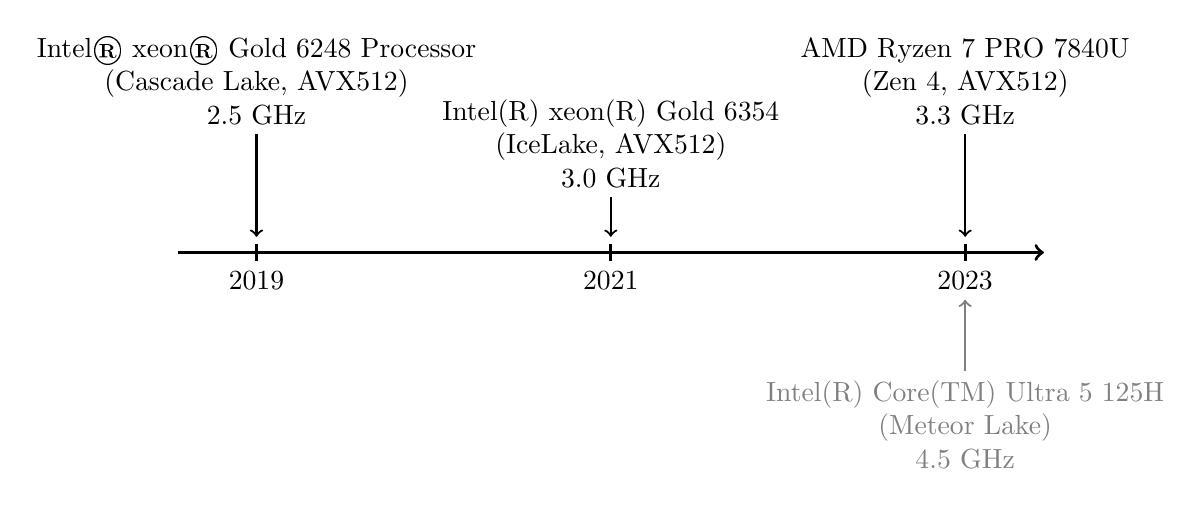
\begin{tikzpicture}[very thick, black]

    %coordinates
    \coordinate (O) at (1,0); % Origin
    \coordinate (F) at (12,0); %End
    \coordinate (P1) at (2,0); %ppti
    \coordinate (P2) at (6.5,0); %groebner
    \coordinate (P3) at (11,0); %mariz+argiope

    %proc
    \draw[<-,thick,color=black] ($(P1)+(0,0.2)$) -- ($(P1)+(0,1.5)$) node [above=0pt,align=center,black] 
    {Intel® xeon® Gold 6248 Processor \\ (Cascade Lake, AVX512) \\ 2.5 GHz};
    \draw[<-,thick,color=black] ($(P2)+(0,0.2)$) -- ($(P2)+(0,0.7)$) node [above=0pt,align=center,black] 
    {Intel(R) xeon(R) Gold 6354 \\ (IceLake, AVX512) \\ 3.0 GHz};
    \draw[<-,thick,color=black] ($(P3)+(0,0.2)$) -- ($(P3)+(0,1.5)$) node [above=0pt,align=center,black] 
    {AMD Ryzen 7 PRO 7840U \\ (Zen 4, AVX512) \\ 3.3 GHz};
    \draw[<-,thick,color=gray] ($(P3)-(0,0.6)$) -- ($(P3)-(0,1.5)$) node [below=0pt,align=center,gray] 
    {Intel(R) Core(TM) Ultra 5 125H \\ (Meteor Lake) \\ 4.5 GHz};

    %main arrow
    \draw[->] (O) -- (F);

    %ticks
    \foreach \x in {2,6.5,11}
    \draw(\x cm,3pt) -- (\x cm,-3pt);
    %labels
    \foreach \i \j in {2/2019,6.5/2021,11/2023}{
    	\draw (\i,0) node[below=3pt] {\j} ;
    }

\end{tikzpicture}

\bigskip
The processor marked in gray corresponds to a machine that does not provide AVX2 so it is only used to check the
correctness of the algorithms and will not appear in the timing comparisons of this document.

\subsection{Profiler}

Timings were measured using a profiler function that resembles the ones provided by FLINT.
It compares the different implementations of given operation and bitsize for the modulus.

\begin{itemize}
    \item explain timings in seconds vs cycle/limb
    \item explain choice of sizes
\end{itemize} 

\section{Vectorization}

\subsection{Auto-vectorization}

\begin{itemize}
    \item explain recent compilers....
    \item explain loop-unrolling
    \item \_\_attribute\_\_((optimize("-fno-tree-vectorize")))
\end{itemize}

\subsection{Single Instruction Multiple Data}

The SIMD instructions form a set of assembly instructions that simultaneously perform an operation on multiple datas stored in registers
of a fixed size allowing to significantly improve the execution speed.

All of the SIMD instructions have a name of the form:
\begin{center} 
    \texttt{<gen><prefix><op><type><size>}
\end{center}

where
\begin{center}
    \begin{minipage}{12cm}
        \begin{itemize}
            \item[\texttt{<gen>}] empty (SSE), v (AVX, AVX2, AVX512)
            \item[\texttt{<prefix>}] empty (unpacked), p (packed)
            \item[\texttt{<op>}] add, sub, mul, sl, sr, \dots
            \item[\texttt{<type>}] l (low part), h (high part), u (unsigned), s (signed), ss (signed with saturation)
            \item[\texttt{<size>}] b (byte - 8 bits), w (word - 16 bits), d (double word - 32 bits), q (quad word - 64 bits), 
            dq (double quad - 128 bits).
        \end{itemize}
    \end{minipage}
\end{center}

\textit{give example}

\bigskip
Rather than directly use these instructions that would lead to writing assembly code, Intel proposes C-style functions
along with vector types that are accessible through the header \texttt{<immintrin.h>}.
They are described in the Intel intrinsics guide\footnote{\url{https://www.intel.com/content/www/us/en/docs/intrinsics-guide/index.html}}.

\bigskip
We mainly used two types of register: 
\begin{itemize}
    \item For AVX2: \texttt{\_\_m256i} which is a 256 bits register that can store up to 4 integers of 64 bits,
    \item For AVX512: \texttt{\_\_m512i} which is a 512 bits register that can store up to 8 integers of 64 bits,
\end{itemize}


\section{Multiplication of $64$ bits integers}

When multiplying two integers, a problem of overflow can arise since the result might be too big to be stored in a $64$ bits word. 
To circumvent this issue, one needs to first split the two integers into two words of a given size and then apply the long multiplication.

\subsection{Long multiplication}
Given two integers $x,y$ both of at most $64$ bits, we start by splitting them into 2 words, one of $k$ bits and the other one of at most $64-k$
bits with $k\leq32$:

\begin{align*}
    x &= x_{hi}\cdot 2^{k} + x_{lo} \\
    y &= y_{hi}\cdot 2^{k} + y_{lo}.
\end{align*}

The long multiplication consists in computing the multiplication of $64$ bits limbs using multiplications and additions of
integers with a lower size.

We compute
\begin{align*}
    r_{lo} &= x_{lo}\cdot y_{lo} \\
    r_{mi} &= x_{lo}\cdot y_{hi} + x_{hi}\cdot y_{lo} \\
    r_{hi} &= x_{hi}\cdot y_{hi}
\end{align*}
then $ab = r_{lo} + (r_{mi} \ll k) + (r_{hi} \ll 2k)$. This formula is mathematically correct but is not used in practice
since it would not fit in a $64$ bits word. 

For a value of $k$ lower than $32$, one has to check that each of the four products computed during the long multiplication can fit in a
64 bits word otherwise it can yield a wrong result.

Furthemore, the addition involved in the computation of $r_{mi}$ can produce an overflow if the inputs are really up to $64$ bits.
For this reason, we restrict the size of $x$ and $y$ to $63$ in practice. 

\subsection{Retrieve the high and the low part of the result}

Since the product $xy$ can have more than 64 bits, but always has at most 128 bits, the output of this operation is usually given as a pair of words of at most 64 
bits such that $xy = (xy)_{hi}\cdot 2^{64} + (xy)_{lo}$.

To do so, one can use the function provided by FLINT \texttt{umul\_ppmm} which is practical since it directly stores the 128-bit result
before splitting it. There are no such intrinsics in AVX2 and AVX512.

In what follows, we consider the two operations:
\begin{itemize}
    \item \texttt{mullo(a,b)}: multiply the $x$-bit integers in $a$ and $b$, producing intermediate $2x$-bit integers, 
    and store the low $x$ bits of the intermediate integers.
    \item \texttt{mulhi(a,b)}: multiply the $x$-bit integers in $a$ and $b$, producing intermediate $2x$-bit integers, 
    and store the high $x$ bits of the intermediate integers.
\end{itemize}

In the AVX2 family, one can find intrinsics for \texttt{mullo} but only for integers up to 32 bits and intrinsics for 
\texttt{mulhi} but only for integers up to 16 bits.

In the AVX512 family, one can only find intrinsics for \texttt{mullo} (up to 64 bits) but it is rather slow on the processors we used.
%% NOTE: except on the zen4 processor

\bigskip
\begin{table}[h!]
    \centering
    \begin{tabularx}{0.7\textwidth} { 
        | >{\centering\arraybackslash}X 
        | >{\centering\arraybackslash}X
        | >{\centering\arraybackslash}X 
        | >{\centering\arraybackslash}X | }
        \hline
        \rowcolor{myGray} 
        Processor & Cascade Lake & IceLake & Zen 4 \\
        \hline
        \cellcolor{myGray} Throughput & 1.5 & 3.0 & 1.0 \\
        \hline
    \end{tabularx}
    \caption{Throughputs of the instruction \texttt{vpmullq zmm, zmm, zmm} for different processors.}
\end{table}

\section{Classic arithmetic operations on vectors}

Each of the following operations have been implemented over 32-bit integers and 64-bit integers.

\subsection{Modular reduction}
\begin{itemize}
    \item \textcolor{orange}{(maybe delayed reduction could be stated as a general principle,
      to circumvent the high cost of reductions;
      it will be possible for some operations but not for others)}
\end{itemize}

\subsection{Addition of two vectors}

Given two vectors $a$, $b$ of $N$ coefficients in $\mathbb{Z}/n\mathbb{Z}$, we compute
\[
a_i + b_i \mod n \qquad \forall i\in \{1,\dots,N\}.
\]

\begin{itemize}
    \item timings
\end{itemize}

\begin{table}[h!]
    \centering
    
    % Proc 1
    \begin{tabular}{|r|*{3}{c c|}}
        \hline
        \rowcolor{myGray} 
        \multicolumn{7}{|c|}{\textsc{Cascade Lake}} \\
        \hline
        \rowcolor{myGray} 
         & t1 & & t2 & & t3 & \\
        \hline
        \cellcolor{myGray} Seq. & xxxx & xxxx & xxxx & xxxx & xxxx & xxxx \\
        \hline
        \cellcolor{myGray} AVX2 & xxxx & xxxx & xxxx & xxxx & xxxx & xxxx \\
        \hline
        \cellcolor{myGray} AVX512 & xxxx & xxxx & xxxx & xxxx & xxxx & xxxx \\
        \hline
    \end{tabular}

    % Proc 2
    \begin{tabular}{|r|*{3}{c c|}}
        \hline
        \rowcolor{myGray} 
        \multicolumn{7}{|c|}{\textsc{IceLake}} \\
        \hline
        \rowcolor{myGray}
         & t1 & & t2 & & t3 & \\
        \hline
        \cellcolor{myGray} Seq. & xxxx & xxxx & xxxx & xxxx & xxxx & xxxx \\
        \hline
        \cellcolor{myGray} AVX2 & xxxx & xxxx & xxxx & xxxx & xxxx & xxxx \\
        \hline
        \cellcolor{myGray} AVX512 & xxxx & xxxx & xxxx & xxxx & xxxx & xxxx \\
        \hline
    \end{tabular}

    % Proc 3
    \begin{tabular}{|r|*{3}{c c|}}
        \hline
        \rowcolor{myGray}
        \multicolumn{7}{|c|}{\textsc{Zen 4}} \\
        \hline
        \rowcolor{myGray}
         & t1 & & t2 & & t3 & \\
        \hline
        \cellcolor{myGray} Seq. & xxxx & xxxx & xxxx & xxxx & xxxx & xxxx \\
        \hline
        \cellcolor{myGray} AVX2 & xxxx & xxxx & xxxx & xxxx & xxxx & xxxx \\
        \hline
        \cellcolor{myGray} AVX512 & xxxx & xxxx & xxxx & xxxx & xxxx & xxxx \\
        \hline
    \end{tabular}
    \caption{Timings in xx and ratios of the modular sum with a modulus of xx bits.}
\end{table}

\subsection{Multiplication of a vector by a scalar or by another vector}

\[
w * b_i \mod n \qquad \forall i\in \{1,\dots,N\}.
\]

\[
a_i * b_i \mod n \qquad \forall i\in \{1,\dots,N\}.
\]

\begin{itemize}
    \item boils down to mult described above
    \item \textcolor{orange}{(here, delaying reductions is basically not possible)}
\end{itemize}

\subsection{Dot product}

For two vectors $u$ and $v$ of $len$ integers of bit size $bitsize \le 32$, and an integer $n$ of some bit size, we want to compute

\[\left(\sum_{i=0}^{len}u_iv_i\right) \mod n\]

To compute the sum of products, we split the integers as described in subsection \ref{sub:split}. Then, we sum separately the three limbs $r_{high}$, $r_{mid}$, $r_{low}$. % TODO: Verify name

\textcolor{orange}{(Here, this is a perfect problem for delaying reductions: e.g. if \(n < 2^{30}\), then a product \(u_iv_i\) is \(< 2^{60}\), so we can sum up to \(2^4 = 16\) terms before doing a reduction)}

\subsubsection{Modular reduction}

The modular is done with \texttt{NMOD2\_RED2} from the flint library. We first regroup the three limbs in two limbs $h$ and $l$ as follows:

\begin{align}
    l &= r_{mid}B &+ \left(r_{high}B^2 + r_{low}\right) \\
    h &= \left\lfloor r_{mid}\frac{B}{2^{64}}\right\rfloor &+ \left\lfloor r_{hi}\frac{B^2}{2^{64}}\right\rfloor &+ c \quad{\text{where $c$ is $1$ if the computation of l overflows and 0 otherwise}}
\end{align}

Because of the cost of this operation, we only reduce at the end, adter the sum. As a consequence, the number of integers we can sum without overflows is limited, and depend of their size.

\begin{proposition}\label{prop:sum}
    For integers of size $\S$, the result of the sum of $2^n$ of such integers is at most $S + n$
\end{proposition}

\begin{proof}
    By induction on $n\in\mathbf{N}$

    \paragraph{Base case: $n = 0$}
    $2^0 = 1$, thus no addition is done and the result has size $S = S + 0 = S + n$. Hence, $\Pi(0)$ is verified.

    \paragraph{Induction}
    Assume for some $i \in \mathbf{N}^*$, $\Pi(i - 1)$ is verified.

    Let $u$ and $v$ be the sums of $2^{i-1}$ integers of size $ S $. By $\Pi(i-1)$, their sizes are at most $S + i - 1$. So the size of $u + v$ is at most $\left(S + i + 1\right) + 1 = S + i$, and $u + v$ is the sum of $2 \cdot 2^(i-1) = 2^i$ integers.
    So $\Pi(i)$ is verified, hence $\Pi(i-1) \Rightarrow \Pi(i)$

    \paragraph{By induction's principle:} $\Pi(0)$ is verified and $\forall i\in\mathbf{N},\ \Pi(i) \Rightarrow \Pi(i+1)$, So
    \begin{displaymath}
        \forall n\in\mathbf{N},\ \Pi(n)\text{ is verified}
    \end{displaymath}
\end{proof}

This value can be computed using \ref{prop:sum}. In our case, because we sum the results of the products of two integers of bit size $bitsize,\ S = 2 bitsize$.

TODO: Max for rhi, rmi and rlo



\section{Butterfly Fast Fourier Transform}

The butterfly refers to an operation that takes place in Cooley-Tukey algorithm (todo:ref), a common algorithm to perfom 
Fast Fourier Transform (FFT), which takes as inputs: $n, w$ a modulus and a scalar of at most 64 bits, and two integers 
$x, y$ in $\mathbb{Z}_n$, and performs the in-place computation:
\[
(x,y) \mapsto (x + w\cdot y \mod n,\ x - w\cdot y \mod n).
\]

Looking at the more global picture, in the FFT algorithm such a butterfly will
be applied to a long vector of different \(x_i, y_i\) but with the same \(w\) and \(n\).


\subsection{Modular multiplication with precomputation}

To take the most of the fixed parameters, V. Shoup\cite{Bos_Stam_2021} introduced a step of precomputations on $w$ and $n$ that will speed up subsequent multiplications by $w \mod n$.

Let $B$ be the maximum bitsize of a word ($B\in \{32, 64\}$). Given $n$ and $w \in \mathbb{Z}_n$, one can compute a scaled approximation 
of $\frac{w}{n}$, which is precisely $$ w_{pre} = \biggl\lfloor\dfrac{w\cdot 2^{B}}{n} \biggr\rfloor.$$

Then, we can run the following algorithm:

for a given vector  , one can compute  as follows:

\begin{algorithm}
    \caption{Shoup modular multiplication}
    \begin{algorithmic}[1]
        \Require $n < B$,
        \Require $0 < w < n$ and its precomputation $0 < w_{pre} < B$,
        \Require $b = (b_1,\dots, b_N)$ with $0 \leq b_i < n \qquad \forall i\in \{1, \dots, N\}$.
        \Ensure $(wb_i \mod n) \qquad \forall i\in{1,\dots, N}$.

        \State Compute $p_{hi}, p_{lo}$ such that $w_{pre} \cdot b_i = p_{hi}\cdot 2^B + p_{lo}$, \Comment{1 \texttt{mulhi}}
        \State $c \gets w\cdot b_i - p_{hi}\cdot n$ \Comment{2 \texttt{mullo}}
        \If {$c \leq n$}
            \State \Return $c-n$
        \Else
            \State \Return $c$
        \EndIf
    \end{algorithmic}
\end{algorithm}

The correctness of this algorithm relies on the definition of $w_{pre}$. 

\begin{proposition}\label{prop:quorem}
For $(x,y) \in \mathbb{Z}\times \mathbb{N}^*$, the quantities $q=\left\lfloor\frac{x}{y}\right\rfloor$ and 
$r=x - \left\lfloor\frac{x}{y}\right\rfloor y$ are respectively the quotient and the remainder in the Euclidian division of $x$ by $y$.
\end{proposition}
    
\begin{proof}
From the definition of the floor of a rational number, we have:
\[
    \left\lfloor\dfrac{x}{y}\right\rfloor \leq \dfrac{x}{y} < \left\lfloor\dfrac{x}{y}\right\rfloor + 1 \Longleftrightarrow
    \left\lfloor\dfrac{x}{y}\right\rfloor y \leq x < \left\lfloor\dfrac{x}{y}\right\rfloor y + y \Longleftrightarrow
    0 \leq x - \left\lfloor\dfrac{x}{y}\right\rfloor y < y.
\]
We then consider $q=\left\lfloor\dfrac{x}{y}\right\rfloor$ and by the uniqueness of the quotient in the Euclidian division with remainder, 
it implies that $x = yq + r$ with $r=x - \left\lfloor\dfrac{x}{y}\right\rfloor y$ and $0 \leq r < y$.
\end{proof}

\begin{proof} (Correctness of the algorithm)
First, using \autoref{prop:quorem}, we have that $w_{pre}= \left\lfloor\frac{w\cdot 2^B}{n}\right\rfloor $ is the quotient in the division 
of $w\cdot 2^B$ by $n$. Thus,
\[
    w\cdot 2^B = w_{pre}\cdot n + r \text{ with } 0 \leq r < n\ \Longleftrightarrow\ w_{pre} = \dfrac{w\cdot 2^B - r}{n}
\]

Thus, by definition of $p_{hi}$,
\[
p_{hi} = \left\lfloor\frac{w_{pre}\cdot b_i}{2^B}\right\rfloor
= \left\lfloor\dfrac{wb_i}{n} - \dfrac{rb_i}{n\cdot 2^B} \right\rfloor.
\]

From the requirements on $r$ and $b_i$ and the previous result, we have that
\[
\left\lfloor\dfrac{wb_i}{n}\right\rfloor - 1 \leq p_{hi} \leq \left\lfloor\dfrac{wb_i}{n}\right\rfloor
\]
and this means that $p_{hi}$ is either $\left\lfloor\frac{wb_i}{n}\right\rfloor - 1$ or $\left\lfloor\frac{wb_i}{n}\right\rfloor$.


It follows that we have
\begin{align*}
\text{either } &c=w\cdot b_i - \left\lfloor\frac{wb_i}{n}\right\rfloor n + n \\
\text{or } &c=w\cdot b_i - \left\lfloor\frac{wb_i}{n}\right\rfloor n.
\end{align*}
Using \autoref{prop:quorem} again, we have $c=wb_i \mod n$ or $c=(wb_i \mod n)+n$, and the last step of the algorithm ensures 
that we retrieve $wb_i \mod n$.
\end{proof}

\begin{remark}
    about mulhi that doesn't need the computation of the carry of low part
\end{remark}


\subsection{Harvey lazy butterfly FFT}

Harvey proposes a strategy\cite{DBLP:journals/corr/abs-1205-2926} to compute the butterfly FFT that allows to save two
modular reductions compared to a basic implementation if one is able to restrict the sizes of the modulus. 

\begin{algorithm}
    \caption{Harvey lazy butterfly FFT}
    \begin{algorithmic}[1]
        \Require $n < B$,
        \Require $0 < w < n$ and its precomputation $0 < w_{pre} < B$,
        \Require $0 \leq x, y < 4n$.
        \Ensure $(x,y) \mapsto (x + w\cdot y \mod n,\ x - w\cdot y \mod n), \qquad 0 \leq x,y < 4p.$

        \If {$x \geq 2p$}
            \State $x \gets x - 2p$
        \EndIf
        \State Compute $p_{hi}, p_{lo}$ such that $w_{pre} \cdot y = p_{hi}\cdot 2^B + p_{lo}$ \Comment{1 \texttt{mulhi}}
        \State $t \gets w\cdot y - p_{hi}\cdot n$ \Comment{2 \texttt{mullo}}
        \State $x \gets x + t$
        \State $y \gets x - t + 2p$
        \State \Return $x,y$
    \end{algorithmic}
\end{algorithm}


\section{Profiling/Benchmarking}


\subsection{Impact of caches} % todo Draft

In the benchmarks, we observes bigger factors than expected between two sizes,
e.g. during the unrolling of non modular dot product. This happen when a vector
become too big to fit in a certain cache, and must be stored in a lower level
cache or in the primary memory. In the previously cited case, it happen for sizes
65536 and 131072 on ppti-gpu-4. % todo detail of calculation



\section{Conclusion}

\appendix
\section{Modular reduction with special primes}

\subsection{Mersenne numbers}

\begin{definition}
    A Mersenne number is of the form $$ M_n = 2^n-1,$$ where $n$ is an integer.

    If $n$ is prime, $M_n$ is also prime and is therefore called a Mersenne prime.
\end{definition}

From this special form, we have for any $n$,
\[
M_n = 0 \mod M_n \Longleftrightarrow 2^n = 1 \mod M_n.
\]

Thus, any integer $x < M_n^2$ can be reduced modulo $M_n$ using only one addition: 
\begin{align*}
x \mod M_n &= x_{hi}\cdot 2^{n} + x_{lo} \mod M_n \\
    &= x_{hi} + x_{lo} \mod M_n.
\end{align*}


\subsection{Generalized Mersenne primes}


\newpage
\bibliographystyle{plain} 
\bibliography{biblio} 
\nocite{*}

\end{document}
